\documentclass[12pt, twoside]{article}
\usepackage[letterpaper, margin=1in, headsep=0.5in]{geometry}
\usepackage[english]{babel}
\usepackage[utf8]{inputenc}
\usepackage{amsmath}
\usepackage{amsfonts}
\usepackage{amssymb}
\usepackage{tikz}

\usepackage{pgfplots}
\pgfplotsset{width=9cm,compat=1.9}

\usepackage{venndiagram}

\usepackage{graphicx}
\usepackage{enumitem}
\usepackage{multicol}

\usepackage{fancyhdr}
\pagestyle{fancy}
\fancyhf{}
\renewcommand{\headrulewidth}{0pt} % disable the underline of the header

\fancyhead[LE]{\thepage}
\fancyhead[RO]{\thepage \\ Name: \hspace{4cm} \,\\}
\fancyhead[LO]{BECA / Dr. Huson / IB Mathematics\\* Unit 3: Probability\\* 13 December 2019}

\begin{document}
\begin{enumerate}
    \subsubsection*{Exam: Probability, Venn diagrams, descriptive statistics, trigonometry}

    \item Given: \\*
        $U = \{\text{the letters in the alphabet}\}$ \qquad
        $A = \{b, e, c, a\}$ \qquad
        $B = \{r, u, l, e, s\}$
        \begin{enumerate}[itemsep=0.7cm]
            \item List the elements of $A \cap B$. \hfill [1 mark]
            \item List the members of $A \cup B$. \hfill [1 mark]
        \end{enumerate} \vspace{0.7cm}

    \item The universal set $U$ is defined as the set of positive integers less than 10. The subsets $A$ and $B$ are defined as follows: \\*[0.25cm]
    $A =$ \{the odd numbers\}
    \qquad $B =$ \{prime numbers\}
    \begin{enumerate}
        \item List the members of $A'$.  \hfill [1 mark] \vspace{1cm}
        \item List the members of $(A \cup B)'$.  \hfill [1 mark] \vspace{1cm}
        \item Place the elements of $A$ and $B$ in the appropriate regions in the Venn diagram below. \hfill [2 marks]
        \begin{center}
            \begin{venndiagram2sets}[tikzoptions={scale=2}]
            \end{venndiagram2sets}U
        \end{center}
        \item List the items in $A \cap B$.  \hfill [1 mark] \vspace{1cm}
        \item If an element is selected at random, what is the probability that it is a member of both sets, ($A \cap B$)? \hfill [1 mark]
    \end{enumerate}

\newpage
    \item For each Venn diagram, shade the area representing the expression. Use pencil.
        \begin{enumerate}
        \item $A \cup B$ \hspace{2cm}
            \begin{venndiagram2sets}
                %\fillANotB
                %\fillB
            \end{venndiagram2sets} \hfill [2 marks]
        \item $A' \cap B$ \hspace{2cm}
            \begin{venndiagram2sets}
            \end{venndiagram2sets} \hfill [2 marks]
        \item $(A \cap B) \cup C$ \hspace{1cm}
            \begin{venndiagram3sets}
            \end{venndiagram3sets} \hfill [2 marks]
            \end{enumerate}

    \item The events $A$ and $B$ are mutually exclusive with $\mathrm P(A)=0.7$ and $\mathrm P(B)=0.2$.
    \begin{enumerate}[itemsep=2.5cm]
        \item Write down $\mathrm P(A \cup B)$. \hfill [1 mark]
        \item Find $\mathrm P(A^\prime \cup B)$. \hfill [1 mark]
    \end{enumerate}

\newpage
    \item The events $A$ and $B$ are independent with $\mathrm P(A)=0.5$ and $\mathrm P(B)=0.8$.
        \begin{enumerate}[itemsep=1.5cm]
            \item Find $\mathrm P(A \cap B)$. \hfill [2 marks]
            \item Find $\mathrm P(A \cup B)$. \hfill [2 marks]
            \item Find $\mathrm P(B | A)$. \hfill [2 marks]
        \end{enumerate} \vspace{1cm}

    \item Given events $A$ and $B$ with $\mathrm P(A)=0.4$, $\mathrm P(B)=0.5$, $\mathrm P(A \cap B)=0.25$.
    \begin{enumerate}
        \item Completely mark the Venn diagram with probabilities for each area. \hfill [2 marks]
        \begin{center}
            \begin{venndiagram2sets}[tikzoptions={scale=1.5}]
            \end{venndiagram2sets}
        \end{center}
        \item Find $\mathrm P(A \cup B)$. \hfill [2 marks] \vspace{1.5cm}
        \item State whether events $A$ and $B$ are independent. Justify your answer.  \hfill [3 marks] \vspace{2cm}
        \item Find $\mathrm P(A | B)$. \hfill [2 marks] 
    \end{enumerate}
    
\newpage
    \item There are 80 athletes playing the following sports:
    \begin{itemize}
      \item 35 play Archery
      \item 44 play Badminton
      \item 39 play Cricket
      \item 16 play Archery and Badminton
      \item 15 play Archery and Cricket
      \item 10 play Badminton and Cricket
      \item 3 play all three of these sports
    \end{itemize}
    Complete the Venn diagram below with the number of students in each region to represent the situation. \hfill [4 marks] 
      \begin{center}
        \begin{venndiagram3sets}[tikzoptions={scale=2.5}]
        \end{venndiagram3sets}U
      \end{center}

\newpage
    \item Forty IB high school students range in age from 15 to 18 years old. The following table shows the frequencies of each age.
        \begin{center}
            \begin{tabular}{|l|r|r|r|r|}
                \hline
                Age (years) & 15 & 16 & 17 & 18\\ 
                \hline 
                Frequency & 5 & $k$ & 15 & 7\\ 
                \hline 
                \end{tabular}      
        \end{center}
        \begin{enumerate}[itemsep=0.8cm]
            \item Calculate the value of $k$. \hfill [1 mark]
            \item Write down the mode. \hfill [1 mark]
            \item Find the value of the range. \hfill [1 marks]
            \item Find the median. \hfill [1 marks]
            \item Find the mean. \hfill [2 marks]
            \item Find the standard deviation. \hfill [2 marks]
        \end{enumerate} \vspace{0.5cm}

    \item A runner records her pace in terms of distance run ($d$) in miles over time ($t$) in minutes during a 4.5 mile run. She models her pace with a linear regression equation $d=at+b$.
        \begin{center}
        \begin{tabular}{|l|c|c|c|c|c|}
            \hline
            minutes ($t$) & 0 & 8 & 15 & 22 & 30 \\ 
            \hline 
            miles ($d$) & 0 & 1.8 & 2.7 & 3.7 & 4.5 \\ 
            \hline 
            \end{tabular}
        \end{center}
        \begin{enumerate}[itemsep=3.5cm]
            \item Find the values of $a$, $b$, and the correlation $r$. \hfill [3 marks]
            \item Explain what the value of $a$ represents in the context of the situation. \hfill [2 marks]
        \end{enumerate}

\newpage
    \item The following diagram shows triangle $ABC$ (not drawn to scale).
    \begin{center}
    \begin{tikzpicture}[scale=1.4, rotate=-15]
        \draw [-, thick] (54:3) node[above right]{$C$}--
        (0,0) node[left]{$A$}--
        (4.5,0) node[right]{$B$}--cycle;
        \node at (0.3, 0.2)[right]{$53^\circ$};
        \node at (4, 0.2)[above left]{$41^\circ$};
        \node at (3.3, 1.7)[below]{$12$};
    \end{tikzpicture}
    \end{center} 
    $BC=12$, $C\hat{A}B=53^\circ$, and $A\hat{B}C=41^\circ$
    \begin{enumerate}
        \item Find the measure of $A\hat{C}B$. \hfill [1 mark] \vspace{3cm}
        \item Find $AC$. \hfill [3 marks] \vspace{5cm}
        \item Find the area of triangle $ABC$. \hfill [3 marks] \vspace{5cm}
    \end{enumerate}
    
\newpage
    \item The histogram below shows the weight $w$ in kilograms for 70 professional football players.

    \begin{center}
        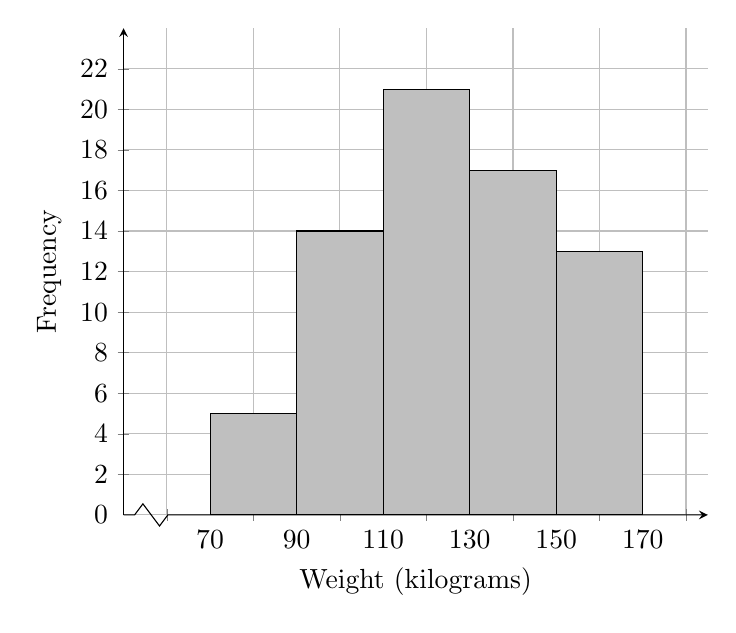
\begin{tikzpicture}
        \begin{axis}[
        xlabel=Weight (kilograms),
        ylabel=Frequency,
        ybar interval=1,
        xmin=60, xmax=195,
        ymin=0, ymax=24,
        xtick={70,90,110,130,150,170,190},
        ytick={0,2,4,6,8,10,12,14,16,18,20,22},
        axis lines = left,
        ymajorgrids=true,
        axis x discontinuity=crunch,
        ]
        \addplot+ [color=black, fill=lightgray]
        coordinates {(80,5) (100,14)
            (120,21) (140,17) 
            (160,13) 
            (180,3)}; %Last pair does not show
        \end{axis}
        \end{tikzpicture}
    \end{center}

    The following is the frequency table for the distribution of $w$. \\[0.25cm]
        \begin{tabular}{|l|c|c|c|c|c|}
        \hline
        HR ($x$) & $70 \leq x < 90$ & $90 \leq x < 110$ & $110 \leq x < 130$ & $130 \leq x < 150$ & $150 \leq x < 170$ \\ 
        \hline 
        Freq & 5 & 14 & 21 & $p$ & 13  \\ 
        \hline 
        \end{tabular}
        \begin{enumerate}
        \item Write down the value of $p$. \hfill [1 mark] \vspace{0.8cm}
        \item Write down the modal class. \hfill [2 marks] \vspace{0.8cm}
        \item A player is selected at random. Find the probability that the athlete weighs less than 110 kilograms. \hfill [2 marks] \vspace{1cm}
        \item Write down the mid-interval value for the class $110 \leq x < 130$. \hfill [1 mark] \vspace{0.8cm}
        \item Hence find an estimate for the
        \begin{enumerate}
            \item mean; \hfill [2 marks] \vspace{0.8cm}
            \item standard deviation. \hfill [2 marks] 
        \end{enumerate}
        \end{enumerate}

    
\newpage
    \item The following diagram shows quadrilateral $ABCD$ (not drawn to scale).
    \begin{center}
    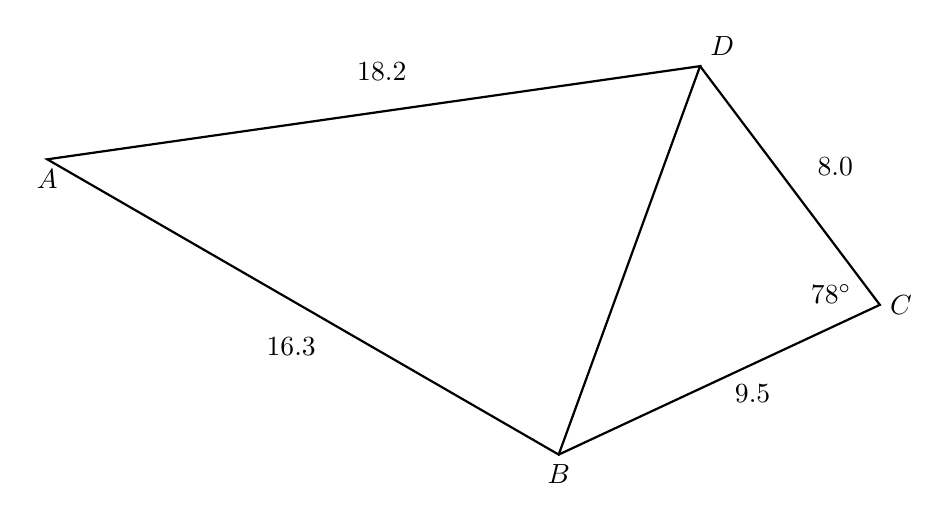
\begin{tikzpicture}[scale=1.5, rotate=-30]
        \draw [-, thick] (100:3.5) node[above right]{$D$}--
        (0,0) node[below]{$B$}--
        (-5,0) node[below]{$A$}--cycle;
        \draw [-, thick] (100:3.5) --
        (55:3) node[right]{$C$}--
        (0,0);             
        \node at (58:2.9)[left]{$78^\circ$};
        \node at (50:1.5)[right]{$9.5$};
        \node at (-2.5,-0.2)[below]{$16.3$};
        \node at (78:3.5)[below]{$8.0$};
        \node at (-3,2.2)[below]{$18.2$};
    \end{tikzpicture}
    \end{center} 
    $AB=16.3$, $BC=9.5$, $CD=8.0$, $AD=18.2$, and $B\hat{C}D=78^\circ$
    \begin{enumerate}
        \item Find $BD$. \hfill [3 marks] \vspace{6cm}
        \item Find $A\hat{B}D$. \hfill [3 marks]
    \end{enumerate}

\newpage
    

\end{enumerate}
\end{document}